\chapter{機能}\label{cha:Function}

本章では、本研究で試作するモータ特性表自動生成ツールの機能について説明する。

Modelica言語で作成したモータのモデルを、OpenModelicaでシミュレーションした時にcsvファイルが出力される。\\
今回試作するモータ特性表自動生成ツールは、OpenModelicaが出力したcsvファイルを入力として読み込み、
モータ特性表を出力として生成する。\\

% \section{ツールの実行方法}\label{zikkou}



% \subsection{ファイル操作}\label{sub:sousa}

% \subsection{実行コマンド}\label{sub:comand}




\section{ツールの機能}\label{kinou}
\subsection{モータ特性表生成}\label{sub:kenkyu_mokuteki}
今回試作したモータ特性表自動生成ツールは、次の9個の要素を持つ特性表と4つのグラフを生成する。

\begin{itemize}
	\item 電圧 V
	\item 始動電流 mA
	\item 停動トルク mNm
	\item 最大効率 \%
	\item 定格トルク mNm 
	\item 定格回転数 rpm
	\item 定格電流 mA
	\item 定格出力 W
	\item 最大回転数 rpm 
\end{itemize}

図\ref{fig:tantai_model}のモデルをシミュレーションした時に、OpenModelicaから出力されるcsvファイルの一部を図\ref{fig:simyu_csv}に、
図\ref{fig:simyu_csv}から作成できるモータ特性表を図\ref{fig:tokuseihyou}に、それぞれ示す。\\

OpenModelicaから出力される
\fboxsep=0pt
\begin{figure}[t]222
	\centering
	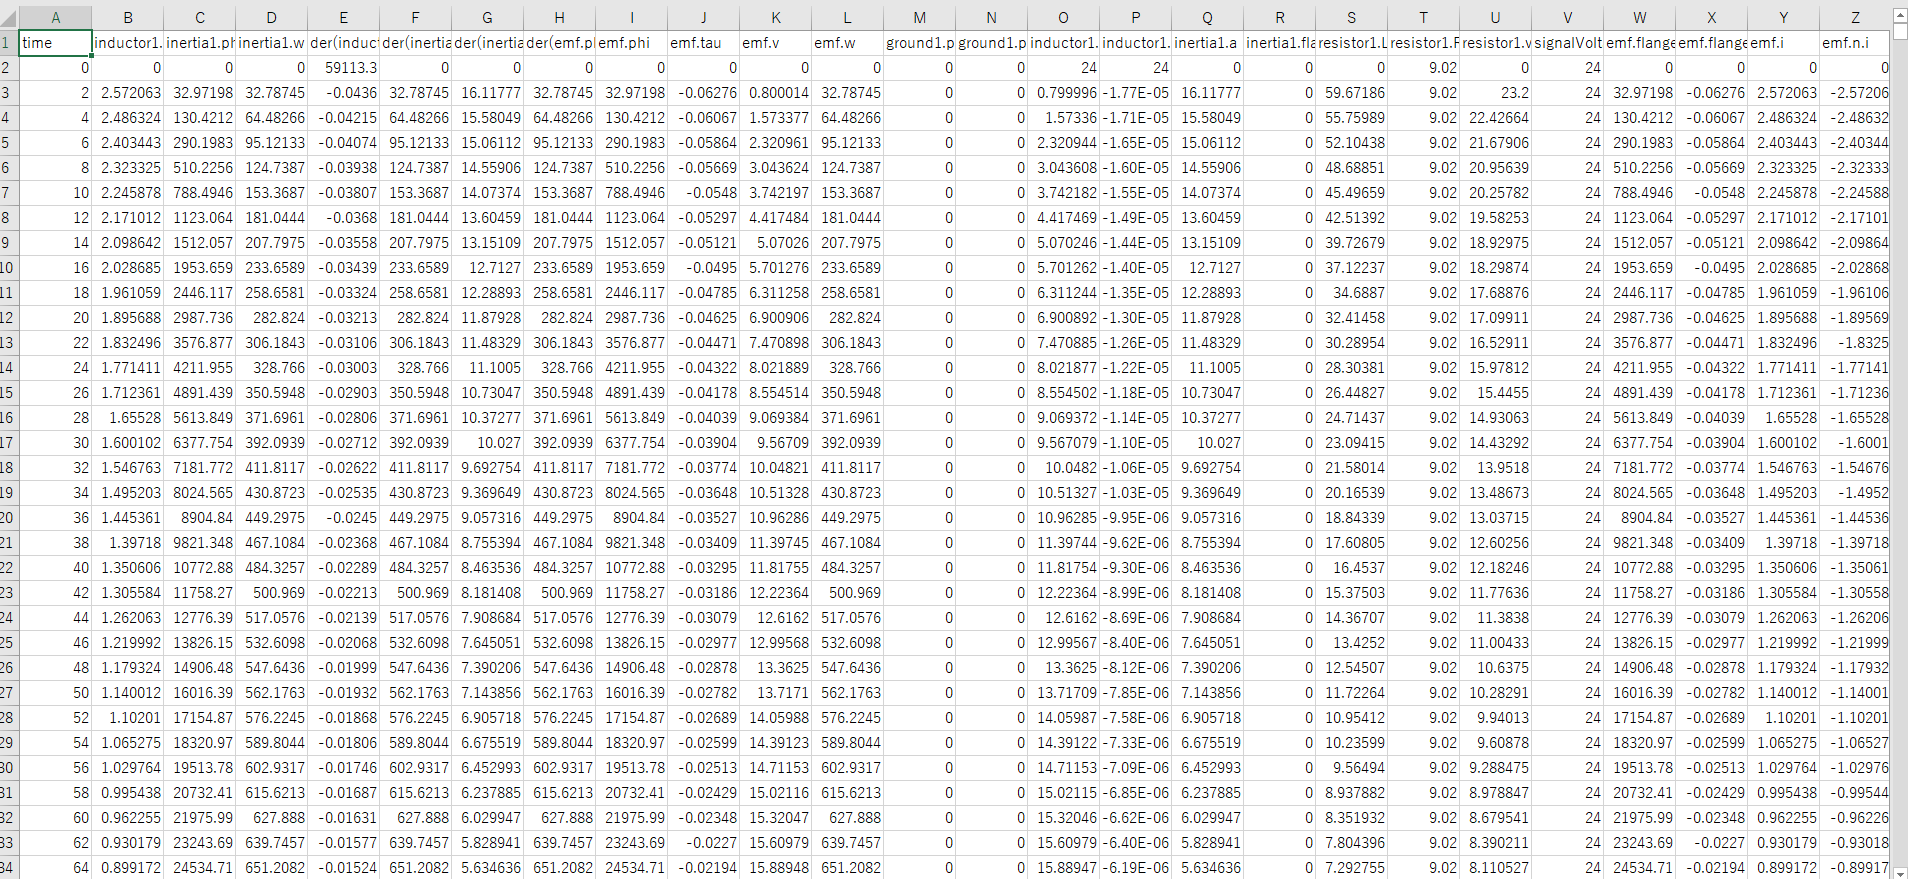
\includegraphics[width=16.5cm,height=9cm]{./Image/simyu_csv.png}
	\caption{図\ref{fig:tantai_model}のシミュレーション結果のcsvファイルの一部}
	\label{fig:simyu_csv}
\end{figure}

\begin{figure}[t]
	\centering
	\fbox{
	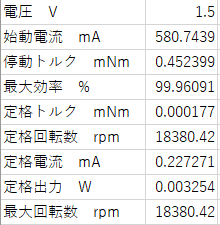
\includegraphics[width=15cm]{./Image/chara_table.png}
	}
	\caption{図\ref{fig:simyu_csv}のcsvファイルから作成したモータ特性表}
	\label{fig:tokuseihyou}
\end{figure}

\subsubsection{電圧}\label{sub:sub:dennatu}
シミュレーション時に印加した値を取る。

\subsubsection{始動電流}\label{sub:sub:sidouden}
始動電流とは、モータの起動時に流れる大きな電流のことである。
モータが起動した後はモータ自体が発電機にもなり、逆起電力を発生するため、モータ・コイル部分にかかる電圧が下がり、電流値も下がる。
したがって、電流値の配列の中で一番大きい値を始動電流とする。
% https://www.tsugawa.co.jp/glossary/ 

\subsubsection{停動トルク}\label{sub:sub:teidoutoruku}
停動トルクとは、モータが出しうる最大トルクで、このトルク以上の負荷がかかれば、モータは停止する値となる。
したがって、トルク値の配列の中で一番大きい値を停動トルクとする。
% https://www.orientalmotor.co.jp/tech/glossary/ta11/

\subsubsection{最大効率}\label{sub:sub:saidaikouritu}
効率は以下の式で算出することができる。

\[
    \mbox{効率} = \frac{\mbox{出力}}{\mbox{入力}}  * 100 
\]
\[
    \mbox{出力} = \mbox{角速度} * \mbox{トルク} 
\]
\[  
    \mbox{入力} = \mbox{電圧} * \mbox{電力} 
\]

各配列を上記の式に当てはめ、繰り返し処理で効率値の配列を作成する。
最大効率は効率値の配列の中で一番大きい値とする。

% https://www.jp-igarashi.com/product/product_motors/curve.html

\subsubsection{定格トルク}\label{sub:sub:teikakutoruku}
最大効率時のトルクを定格トルクという。
したがって、トルク値の配列の中で、最大効率のある効率値の配列の添字と同じ位置にある値が定格トルクとなる。


% http://www.sagamimicro.co.jp/product/aboutusage.html

\subsubsection{定格回転数}\label{sub:sub:teikakukaiten}
最大効率時の回転数を定格回転数という。
回転数は以下の式で算出できる。

\[
    \mbox{回転数} = \frac{30 * \mbox{角速度}}{\pi}   
\]

したがって、一度繰り返し処理で角速度を回転数に変換し、回転数値の配列の中で、最大効率のある効率値の配列の添字と同じ
位置にある値が定格回転数となる。

% https://mathwords.net/kaitensu

\subsubsection{定格電流}\label{sub:sub:teikakuden}
定格電流とは、モータに定格トルクがかかっているときの電流値である。
したがって、電流値の配列の中で、定格トルクのあるトルク値の配列の添字と同じ位置にある値が定格電流となる。

% http://fa-faq.mitsubishielectric.co.jp/faq/show/18504?category_id=1937&site_domain=default

\subsubsection{定格出力}\label{sub:sub:teikakusyutu}
定格出力とは、定格動作点における出力の値である。
定格出力は以下の式で算出できる。

\[
    \mbox{定格出力} = \mbox{定格回転数} * \mbox{定格トルク} *  \frac{2\pi}{60}
\]
% \ref{sub:sub:teikakukaiten}章で求めた定格回転数と\ref{sub:sub:teidoutoruku}章で求めた定格トルクを
% http://www.nidec-servo.com/jp/digital/pdf/A_technique.pdf


\subsection{エラー表示}\label{error}
